\documentclass[Orbiter Developer Manual.tex]{subfiles}
\begin{document}

\section{Orbiter 2D Graphics}
When doing a low level add-on development for the Orbiter, you need to access to a surfaces from time to time. This sections gives you a brief introduction to overall working of surfaces in the Orbiter and computer graphics in general. The GPU can read from some surfaces and write to an other. The main CPU also has a limited access to some surfaces. Since a modern computer processing in multi-threaded an invalid access to a bad surface can cause render pipeline stalls. Common rule of thumb is that one surface cannot be written in by both GPU and CPU.\\

\begin{figure}[H]
  \centering
  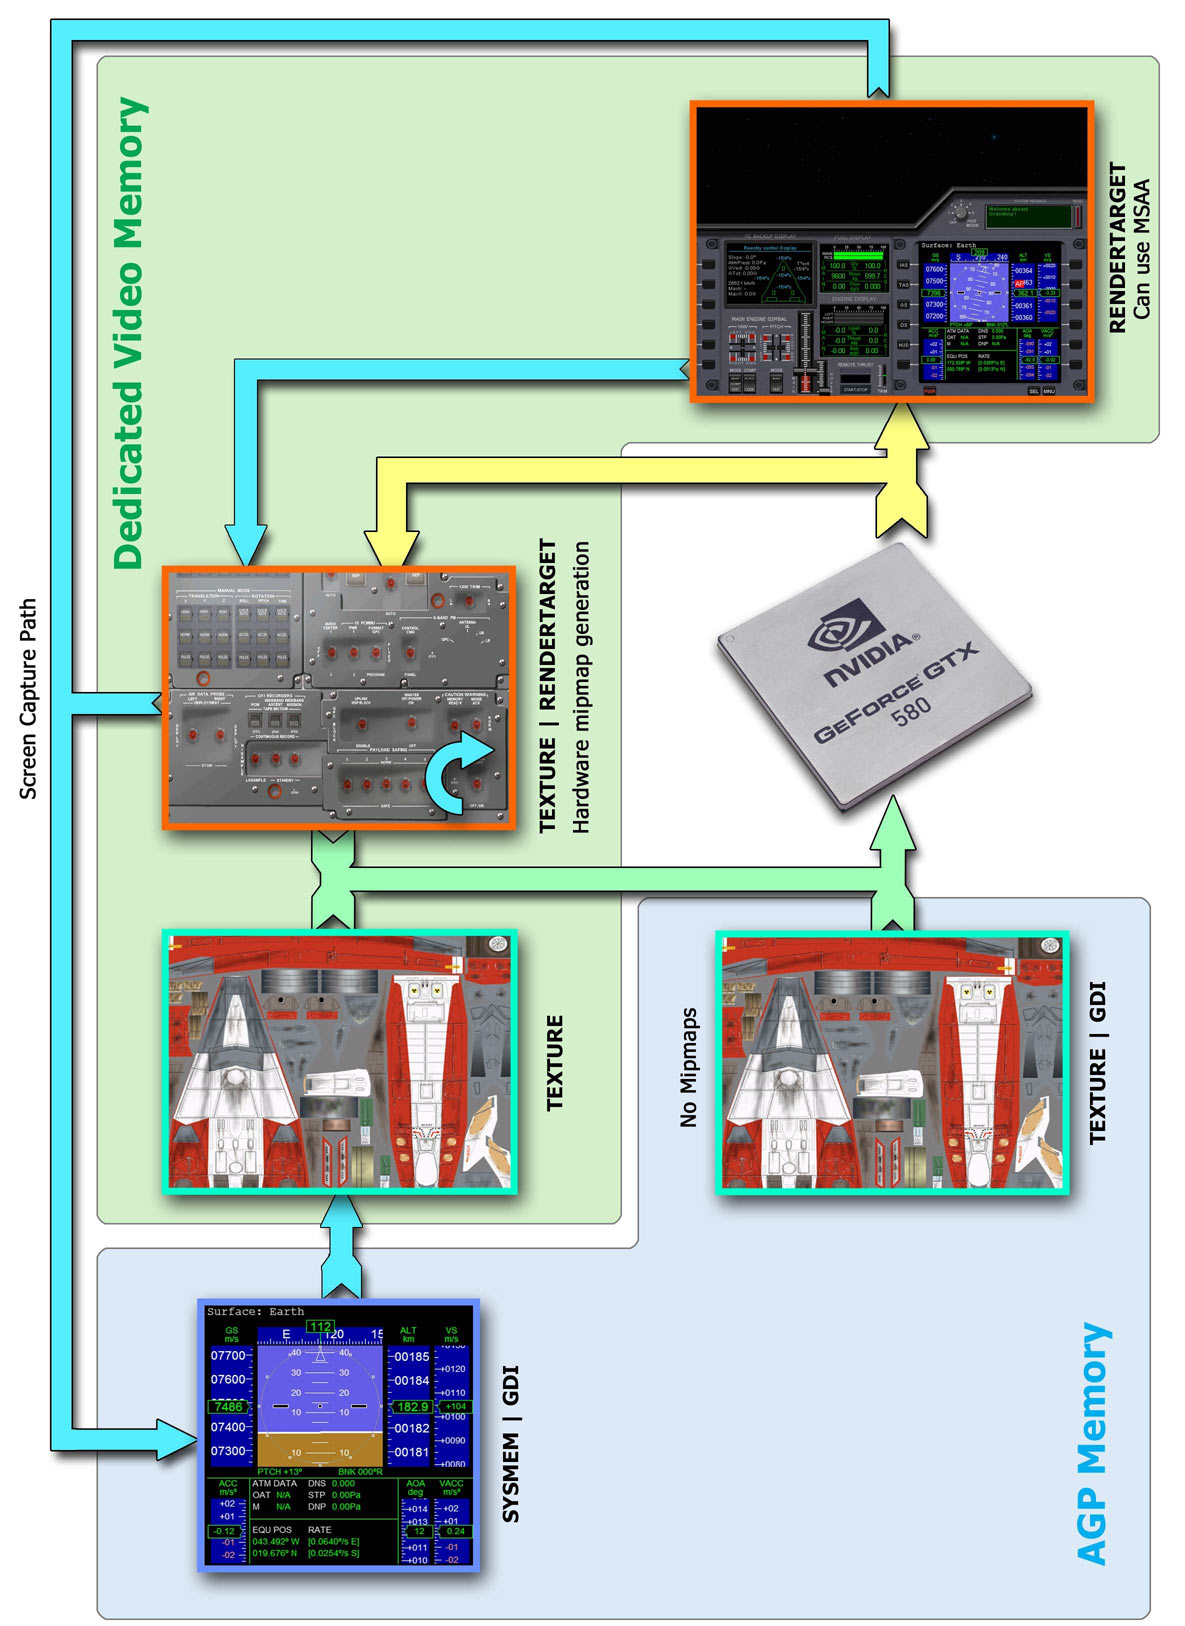
\includegraphics[width=0.8\hsize]{2dflow.jpg}
\end{figure}

\subsection{Flow chart}
When looking at the graphics flow chart from a previous page you can focus your attention to the GPU and how it is positioned relative to the five different surfaces in the schematics. The GPU is the primary execution unit that creates almost all of the graphics we see in the Orbiter. Rendering Meshes, drawing with the Sketchpad and executing commands like \textit{oapiBlt}, \textit{oapiClearSurface} and \textit{oapiColourFill} functions are all done with the GPU. The main flow of graphics in the schematics is from the bottom to the top.\\

The GPU can only draw/render graphics in a surface created as \textsc{RENDERTARGET}. The yellow pathway in the schematics represents that path (i.e. Output from the GPU). Also, any surface that is being read by the GPU must be a \textsc{TEXTURE}. This is shown as a green pathway in the schematics (i.e. Input to the GPU). When \textit{oapiBlt} is used to copy graphics along green and yellow pathways, stretching and color-keying are supported. However, for such operations a use of Sketchpad is recommended especially if there is a higher quantity of copy operations per target.\\

In addition to the GPU there also exists a resource management unit that can transfer data between various graphics resources, however the transfer is limited to a simple plain copy operation only. Surface formats must be identical in source and destination. Color operations such as alpha-blending, color-keying or stretching are not supported. These options are presented via the blue pathway in the schematics and the copy operations can be done by using oapiBlt. The "screen capture pathway" has a special requirements those are discussed later on.\\

Orbiter API calls \textit{oapiCreateSurfaceEx} and \textit{oapiLoadSurfaceEx} can be used for creating a surfaces or loading graphics directly into a specific type of a surface. 
\textsc{SKETCHPAD} flag is identical to \textsc{RENDERTARGET} flag.

\subsection{Rendering to a Texture}
The \textsc{RENDERTARGET | TEXTURE} is the most versatile surface there is and likely the most common user allocated surface in the Orbiter. It can be used for both reading and writing by the GPU. If combined with \textsc{MIPMAPS} flag a full chain of mipmaps are created. The mipmaps are automatically regenerated by hardware when being used as a texture after the main/top surface level has been modified by any operation. So, one can assign this kind of surface directly into a mesh and draw onto it.\\

The small curved arrow in a lower-right corner of the surface indicates that the surface can be used for in-surface blitting (\textsl{i.e. the same surface can be a source and a target at the same time and the rects can overlap}), but that is limited to a simple copy rect operation with \textit{oapiBlt}. That is not a native graphics feature and it is actually done with two copy operations through a temporary surface. The old \textit{oapiCreateSurface} and \textit{oapiCreateTextureSurface} will create a \textsc{RENDERTARGET | TEXTURE} and the later will also add \textsc{MIPMAPS} flag and the format is XRGB in both cases. 

\subsection{Rendertarget}
The plain vanilla \textsc{RENDERTARGET} is a single layer surface (e.g. no mipmap support). The only specialty in this surface is MSAA (Multi-Sample-Anti-Alias) which can be enabled by adding \textsc{ANTIALIAS} flag to a surface creation. The level of anti-aliasing will depend on Launchpad configurations. 3D rendering ability can be enabled for any \textsc{RENDERTARGET} by adding \textsc{RENDER3D} flag. This will also work for \textsc{RENDERTARGET | TEXTURE}.

\subsection{Texture}
The old good \textsc{TEXTURE} is most common surface and it's mainly used a by meshes and are automatically loaded by the Orbiter. If \textsc{MIPMAPS} flag is specified during loading or surface creation, a full chain of mipmaps are created even if the file doesn't have any. Also \textsc{NOMIPMAPS} flag will tell the texture loaded to reject any mipmaps the file might have. If neither flag is defined then the outcome is defined by the file being loaded. This surface cannot be written in by GPU.

\subsection{Dynamic texture}
\textsc{TEXTURE | GDI} is a dynamic surface located in AGP memory and can be updated by the CPU. Also can be used for drawing by GDI in other words \textit{oapiGetSurfaceDC} works with this surface but should be avoided due to it's platform specific nature. There are no mipmap support in this surface type. If the surface data is being accessed by CPU its write only access. Always uncompressed format XRGB.

\subsection{System memory surface}
\textsc{SYSMEM | GDI} is a graphics surface located in a system memory or in an AGP memory depending on implementation.  \textit{oapiGetSurfaceDC} also works with this surface and the surface data can be accessed by CPU for reading and writing. No mipmap support. If the entire surface (not a sub-rect) is copied to a \textsc{TEXTURE|MIPMAPS} surface created with \textit{oapiCreateSurfaceEx} then a full chain of mipmaps are created in destination. Although, the level of hardware support and therefore speed may wary depending on implementation. 

\subsection{Surface decompression}
There are ways to request a texture decompression and in some cases it will happen automatically. As an example \textsc{RENDERTARGET} can't be compressed, therefore, if a texture is being loaded directly into such a surface then a decompression is automatically applied. By default the format is XRGB but it can be user controlled by applying \textsc{ALPHA} flag to decompress ARGB. Decompression of a regular texture can be enabled by passing \textsc{DECOMPRES} flag.\\

Addition of 'D' charter after the texture name in a mesh file will trigger decompression into XRGB format.

\end{document}
